% Licencia y derechos: consulte ../../LICENSE-CC-BY-4.0.
% Las figuras y demás materiales de terceros pueden tener derechos separados y deben identificarse.

\chapter{Amplificadores de potencia} %p241

Los amplificadores de potencia son etapas amplificadoras que tienen que manejar una potencia relativamente elevada. Debido justamente a las señales grandes, los transistores ya \underline{no trabajan en forma lineal}; consecuentemente el modelo lineal del transistor deja de ser una descripción precisa del dispositivo y para mayor exactitud se acude al \underline{análisis gráfico}. Otra consecuencia es que se produce una \underline{distorsión de la señal}, la cual debe ser evitada y superada en lo posible pues se quiere reproducir la señal de entrada en forma lineal. 

Debido también a las grandes potencias desarrolladas, los dispositivos utilizados \underline{tienden a recalentarse}; los \underline{sumideros térmicos} permiten disipar más efectivamente el calor generado en el dispositivo. Además aquí es particularmente importante prestarle toda la atención a los \underline{valores límites de voltaje, corriente y potencia del dispositivo}, para asegurar que no se excedan. 

Finalmente se plantea el interés y la necesidad de un buen \underline{rendimiento}, es decir, un \underline{uso eficiente de la fuente de poder}, para reducir su tamaño y costo al mínimo posible.

\section{Generalidades} %p241

La potencia instantánea disipada en un dispositivo es igual al producto de voltaje y corriente, $p = vi$.

Para señales periódicas, es preferible hablar de la potencia promedio durante un período:

\begin{equation}
	\bar{P} = \frac{1}{T} \int_0^T vi \, dt
\end{equation}

Entonces:

\begin{equation}
	\bar{P} = V I \cos \varphi
\end{equation}

donde $\varphi$ representa el desfase entre el voltaje y la corriente, cuyas amplitudes son $V$ e $I$ respectivamente. Para cargas resistivas, lo típico en nuestros casos, $\varphi = 0$. Alternativas para expresar lo mismo:

\begin{equation}
	\bar{P} = I_{\text{ef}} V_{\text{ef}} = I_{\text{ef}}^2 R = \frac{V_{\text{ef}}^2}{R}
\end{equation}

donde la señal eficaz, $I_{\text{ef}}$ o $V_{\text{ef}}$, se encuentra de la siguiente ecuación:

\begin{equation} \label{eq:potencia-forma-alternativa}
	X_{\text{ef}} = \left( \frac{1}{T} \int_0^T x^2 dt \right)^{1/2}
\end{equation}

En la siguiente tabla se indica el valor eficaz para varios tipos de señal.

\begin{tabular}{cccc}
	\hline
	\textbf{Descripción} & \textbf{Expresión} & \textbf{Dibujo} & \textbf{Valor Eficaz} \\
	\hline
	1. Sinusoidal & $X_p \sin \omega t$ & Fig. \ref{fig:potencia_dibujo-seno} & $X_{\text{ef}} = \frac{X_p}{\sqrt{2}}$ \\
	\hline
	2. Nivel DC & $X_{\text{cc}}$ & Fig. \ref{fig:potencia_dibujo-dc} & $X_{\text{ef}} = X_{\text{cc}}$ \\
	\hline
	3. Onda Cuadrada & $\pm X_{\text{cc}}$ & Fig. \ref{fig:potencia_dibujo-onda-cuadrada} & $X_{\text{ef}} = X_{\text{cc}}$ \\
	\hline
	4. Onda Triangular & Valor pico $X_p$ & Fig. \ref{potencia_dibujo-onda-triangular} & $X_{\text{ef}} = \frac{X_p}{\sqrt{3}}$ \\
	\hline
\end{tabular}

\begin{figure}[h]
	\centering
	\subfloat[Sinusoidal]
	{
		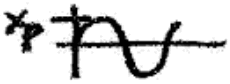
\includegraphics[width=0.16\linewidth]{_fig/potencia_dibujo-seno.png}
		\label{fig:potencia_dibujo-seno}
	}
	\subfloat[Nivel DC]
	{
		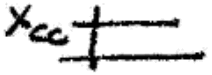
\includegraphics[width=0.16\linewidth]{_fig/potencia_dibujo-dc.png}
		\label{fig:potencia_dibujo-dc}
	}
	\subfloat[Onda Cuadrada]
	{
		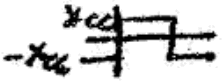
\includegraphics[width=0.16\linewidth]{_fig/potencia_dibujo-onda-cuadrada.png}
		\label{fig:potencia_dibujo-onda-cuadrada}
	}
	\subfloat[Onda Triangular]
	{
		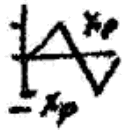
\includegraphics[width=0.10\linewidth]{_fig/potencia_dibujo-onda-triangular.png}
		\label{potencia_dibujo-onda-triangular}
	}
	\caption{Dibujos complemento}
	\label{fig:potencia_dibujos}
\end{figure}

Por lo general, nosotros vamos a trabajar con señales sinusoidales; para este tipo de señal, la ecuación \ref{eq:potencia-forma-alternativa} queda:

\[
\bar{P} = V_p I_p / 2
\]

Con esta relación sencilla se puede determinar la potencia típica entregada por los circuitos más conocidos.

\subsection{Ejemplo}

Un amplificador EC de pequeña señal con punto de operación óptimo (Figura 6.3). Si $V = 10V$ entonces $V_{CE} \approx 5V$; deja que $I_C = 5 \text{mA}$. Para la misma variación de la salida sin distorsión: $V_p \approx 5V$, $I_p \approx 5 \text{mA}$, y \( \bar{P} = (5V)(5 \text{mA})/2 = 12.5 mW \). Esto representa una potencia relativamente pequeña. Ver figura de las características de salida para este caso, la Figura \ref{fig:potencia_amplificador-ec_senal-pequena}.

\begin{figure}[h]
	\centering
	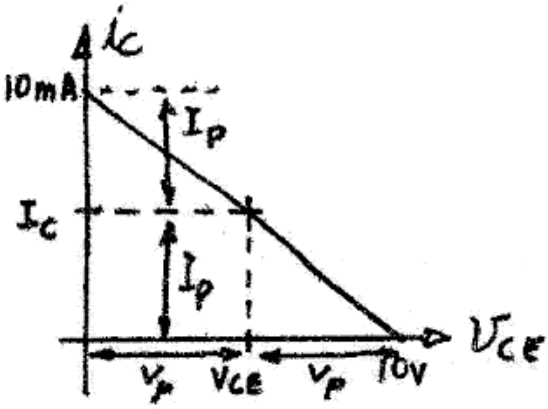
\includegraphics[width=0.8\linewidth]{_fig/potencia_amplificador-ec_senal-pequena.png}
	\caption{Amplificador EC, Señal Pequeña}
	\label{fig:potencia_amplificador-ec_senal-pequena}
\end{figure}

\subsection{Ejemplo}

Un amplificador operacional de propósito general, como el 741, operando a su máxima capacidad con fuentes de $\pm$ 15V. El fabricante nos indica en una tabla que con una carga de $R1 = 1\,k\Omega$, $V_o(\text{max})$ (pico a pico) $= 25\,V$. Entonces,

\[
P = \left(\frac{V_o(\text{pico a pico})}{2\sqrt{2}}\right)^2 / R1 = \left(\frac{25}{2\sqrt{2}}\right)^2 / 1\,k\Omega = 78\,\text{mW}
\]

Esto todavía representa una potencia relativamente pequeña.

Comercialmente se consiguen circuitos integrados, como el LM383 de National, que pueden entregar $7\,W$ a una carga de $4\,\Omega$, y circuitos híbridos, como el TIXH601 de Texas Instruments, que pueden entregar $100\,W$, con unas conexiones externas tan sencillas como cualquier amplificador operacional. Estos representan una solución fácil y directa para un gran número de aplicaciones.

Con ellos se mantiene vigente las preocupaciones de estabilidad térmica. Típicamente se utiliza la retroalimentación para reducir la distorsión y están diseñados para dar un rendimiento elevado de la potencia entregada por la fuente.

Para casos especiales y en los diseños con algunos años de antigüedad se utilizan las configuraciones hechas en base a transistores; además las etapas de salida internas a los circuitos integrados e híbridos están compuestas de estas configuraciones. Por lo tanto estaremos trabajando sobre todo con configuraciones transistorizadas.

Generalmente los transistores de potencia son fabricados con dimensiones grandes para así permitirles aguantar mejor las corrientes grandes que por ellos van a circular. Esto conlleva a que el \( \beta \) y el \( f_T \) sean pequeños.

En la característica de salida típica de un transistor de potencia que se muestra en la Figura \ref{fig:potencia_amplificador-ec_senal-grande}, se observa que las distancias entre las curvas no son iguales, lo cual es indicativo de que \( \beta \) no es una constante.

\begin{figure}[h]
	\centering
	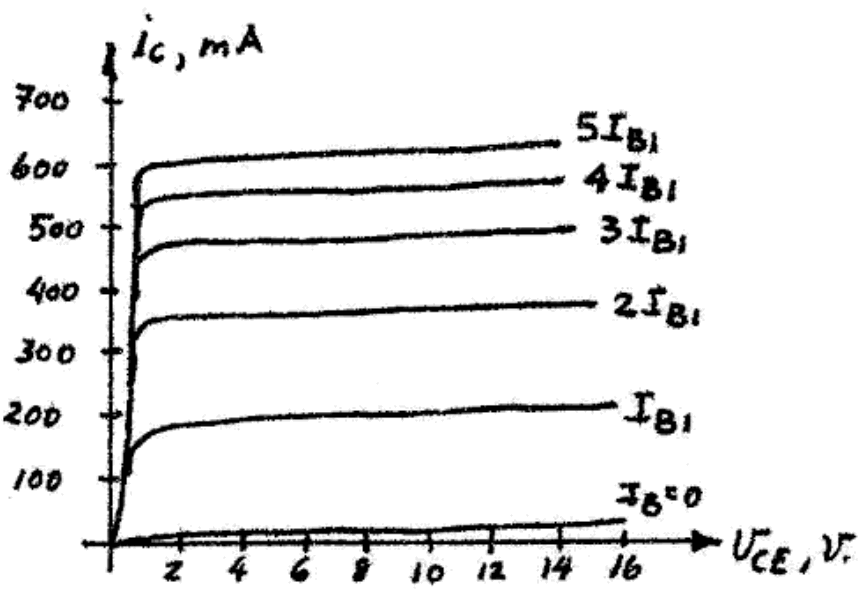
\includegraphics[width=0.8\linewidth]{_fig/potencia_amplificador-ec_senal-grande.png}
	\caption{Amplificador EC, Señal Grande}
	\label{fig:potencia_amplificador-ec_senal-grande}
\end{figure}

\section{Conceptos de potencia disipada en el dispositivo con y sin señal y el rendimiento del circuito} %p244

\begin{figure}[h]
	\centering
	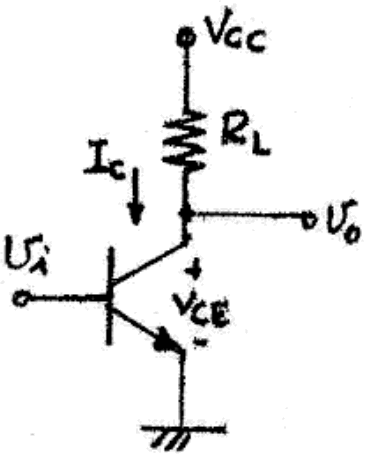
\includegraphics[width=0.8\linewidth]{_fig/potencia_amplificador-ec.png}
	\caption{Amplificador EC}
	\label{fig:potencia_amplificador-ec}
\end{figure}

Para apreciar algunos conceptos de interés, se analiza la configuración EC de la Figura \ref{fig:potencia_amplificador-ec}, la cual se encuentra en la región activa. Cuando no hay señal de entrada, la potencia entregada por la fuente de poder es \( P_{CC} = V_{CC} I_C \), la potencia disipada en la resistencia es \( I_C^2 R_L \), y la \textbf{potencia disipada en el transistor} es:

\begin{equation} \label{potencia_pd1}
	P_D = P_{CC} - P_{RL} = V_{CC} I_C - I_C^2 R_L
\end{equation}

Cuando hay una señal de entrada, la potencia entregada por la fuente es:

\[
P_{CC} = \frac{1}{T} \int_0^T V_{CC} (I_C + I_m \sin \omega t) dt = V_{CC} I_C
\]

es decir, no varía. La potencia disipada en la resistencia viene dada por:

\[
P_{RL} = \frac{1}{T} \int_0^T (I_C + I_m \sin \omega t)^2 R_L dt = \frac{1}{T} \int_0^T (I_C^2 + 2 I_C I_m \sin \omega t + I_m^2 \sin^2 \omega t) R_L dt
\]
\[
P_{RL} = I_C^2 R_L + \frac{1}{T} \int_0^T I_m^2 R_L \sin^2 \omega t \, dt = I_C^2 R_L + \frac{I_m^2 R_L}{2}
\]

La componente: \( P_O = \frac{I_m^2 R_L}{2} \) es la que surge como consecuencia de la variación de la señal de entrada y depende directamente de ésta, y por eso se considera la potencia útil, la potencia de salida. 
En todo caso, ahora la potencia disipada en el transistor ha disminuido, ya que:

\begin{equation} \label{potencia_pd2}
	P_{D}' \text{con señal} = P_{CC} - I_C^2 R_L - \frac{1}{2} I_m^2 R_L
\end{equation}

Se hace notar que para este tipo de polarización, en la región activa (y por lo tanto Clase A), el transistor disipa la mayor cantidad de potencia bajo condiciones de reposo.	El \textbf{rendimiento} de una configuración viene dado por:

\begin{equation}
	\eta = \frac{P_{sal}}{P_{fuente}}
\end{equation}

donde:

\begin{itemize}
	\item \(P_{sal}\) representa la potencia útil de salida
	\item \(P_{fuente}\) representa la potencia entregada por la(s) fuente(s)
	\item \(P_{CC}\) en la ecuaciones \ref{potencia_pd1} y \ref{potencia_pd2}
\end{itemize}

El \textbf{rendimiento máximo}, \(\eta(\text{max})\), se calcula para cuando se desarrolla la máxima potencia de salida sin distorsión, \(P_{sal}(\text{max})\).

El \textbf{rendimiento máximo óptimo}, \(\eta(\text{opt})\), representa una mejora pues implica que el punto de operación es óptimo y por lo tanto hay más potencia de salida.
hro
Finalmente, se determina el \textbf{rendimiento máximo óptimo ideal}, \(\eta(\text{ideal})\), para un tipo general de amplificador donde se asumen condiciones ideales. Se determina el rendimiento máximo óptimo ideal para el circuito tipo de la Figura \ref{fig:potencia_amplificador-ec} (Clase A, carga resistiva), con el punto de operación en su punto óptimo \((V_{CE} = V_{CC}/2)\) y con condiciones idealizadas de \(V_{CE(\text{sat})} = 0\,V\), e \(I_C(\text{corte}) = 0\,A\), entonces dado una señal sinusoidal de entrada, se tiene:

\[
P_{sal}(\text{max}) = I_P V_P / 2 = I_C V_{CE} / 2 = I_C V_{CC} / 4
\]

Después: \( \eta(\text{ideal}) = \left( I_C V_{CC}/4 \right) / I_C V_{CC} = 1/4 \), es decir, un rendimiento del \( 25\% \). Por cada \( 10 \text{Watts} \) de la fuente, sólo \( 2.5 \text{Watts} \) se disipa como potencia útil. El resto se disipa en el transistor o en la resistencia como potencia "desperdiciada" de corriente continua.

Esta configuración presenta un gran defecto ya que la fuente de poder está disipando potencia, aún en la ausencia de una señal de entrada. Sería mejor un sistema cuya fuente de poder entrega potencia sólo cuando se va a entregar potencia útil a la carga.

\section{El transformador en los amplificadores de potencia} %p246

El transformador es de utilidad para: 

\begin{itemize}
	\item[a)] aumentar el rendimiento de los amplificadores Clase A,
	\item[b)] aumentar la variación de tensión pico a pico en la carga sin necesidad de una fuente de tensión elevada, y 
	\item[c)] permitir acople de impedancias.
\end{itemize}

\begin{figure}[h]
	\centering
	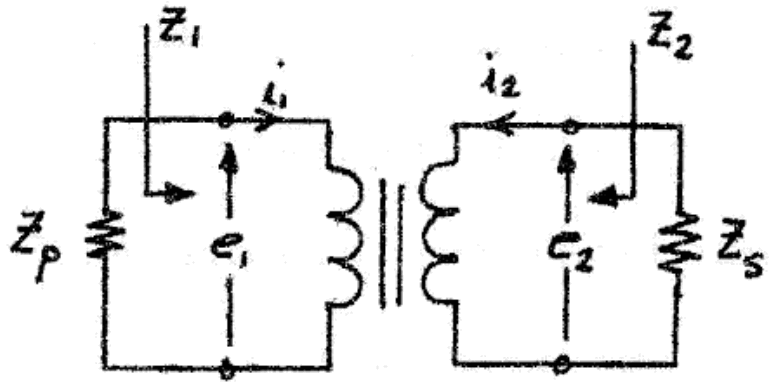
\includegraphics[width=0.8\linewidth]{_fig/potencia_transformador.png}
	\caption{Transformador y su relación}
	\label{fig:potencia_transformador}
\end{figure}

En la Figura \ref{fig:potencia_transformador} se identifican los terminales del transformador y se consiguen las siguientes relaciones, donde \(n\) es el número de vueltas en el primario y \(n_2\) el número del secundario:

\begin{equation}
	\frac{e_1}{e_2} = \frac{n_1}{n_2} = n
\end{equation}

\begin{equation}
	\frac{i_1}{i_2} = -\frac{1}{n}
\end{equation}

De donde:

\begin{equation}
	Z_1 = n^2 Z_s \quad \text{y} \quad Z_2 = \frac{Z_p}{n^2}
\end{equation}

El modelo T equivalente del transformador, dado en la Figura \ref{fig:potencia_transformador-t-equivalente}, es el de mayor utilidad en los circuitos electrónicos. En esta figura, a la izquierda, \(L_{11}\) representa la inductancia en la primaria, \(L_{22}\) representa la inductancia de la secundaria, \(M\) representa la inductancia mutua, y \(K\) el coeficiente de acoplamiento.

\begin{figure}[h]
	\centering
	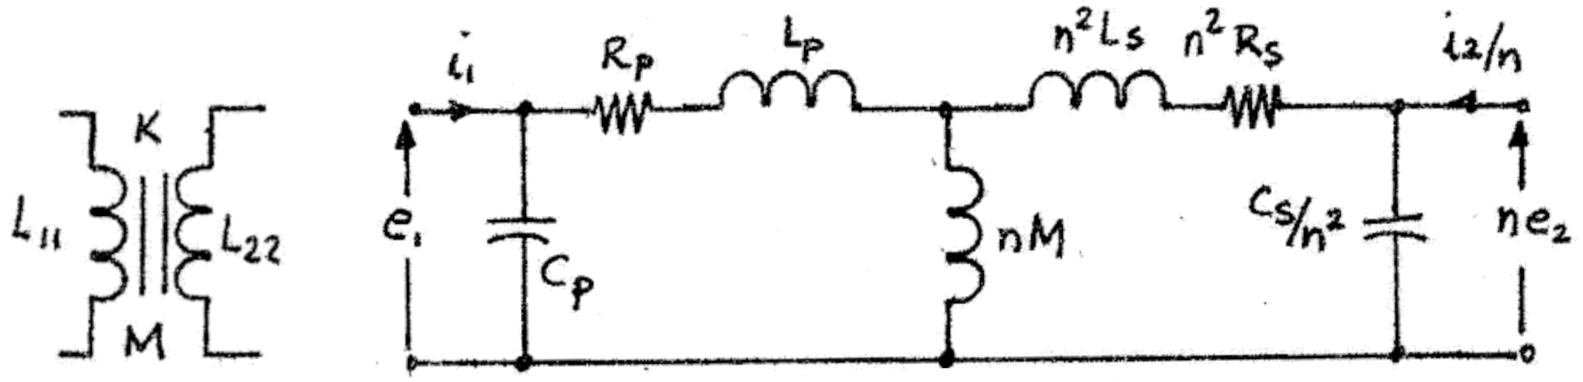
\includegraphics[width=0.8\linewidth]{_fig/potencia_transformador-t-equivalente.png}
	\caption{Modelo T equivalente del transformador}
	\label{fig:potencia_transformador-t-equivalente}
\end{figure}

En el modelo T equivalente, \(R_p\) representa la resistencia de la primaria, \(R_s\) la resistencia de la secundaria, \(n^2 R_s\) la resistencia de la secundaria referida a la primaria, \(L_p\) representa la inductancia de fuga de la primaria, \( L_p = (1 - K) L_{11} \) y \(L_s\) es la inductancia de fuga de la secundaria,	\( L_s = (1 - K) L_{22} \).

Para un análisis en la frecuencia del transformador se incluye sólo algunos elementos del modelo de acuerdo al rango de frecuencia correspondiente al análisis, como cuando se analiza un amplificador: 

\begin{itemize}
	\item[a)] A frecuencias medias se elimina todo lo reactivo y queda el modelo de la Figura \ref{fig:potencia_modelo-transformador-a};
	\item[b)] A frecuencias bajas las capacitancias son despreciables por presentar una reactancia elevada, y las inductancias de fuga son despreciables por presentar una reactancia muy pequeña; queda el modelo de la Figura \ref{fig:potencia_modelo-transformador-b};
	\item[c)] A a frecuencias elevadas la reactancia \(nM\) es muy elevada y se desprecia su efecto; queda el modelo de la Figura \ref{fig:potencia_modelo-transformador-c}.
\end{itemize}

\begin{figure}[h]
	\centering
	\subfloat[A]
	{
		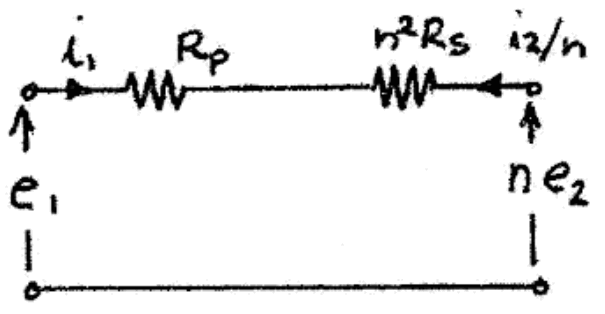
\includegraphics[width=0.32\linewidth]{_fig/potencia_modelo-transformador-a.png}
		\label{fig:potencia_modelo-transformador-a}
	}
	\subfloat[B]
	{
		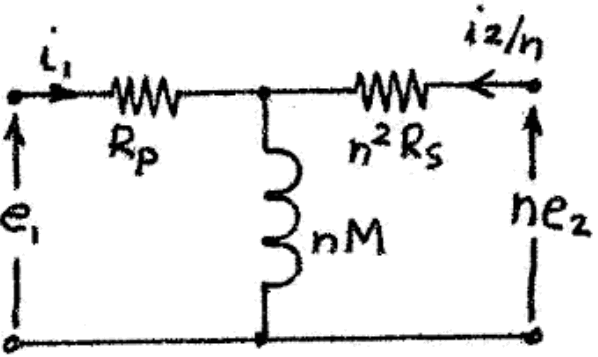
\includegraphics[width=0.32\linewidth]{_fig/potencia_modelo-transformador-b.png}
		\label{fig:potencia_modelo-transformador-b}
	}
	\subfloat[C]
	{
		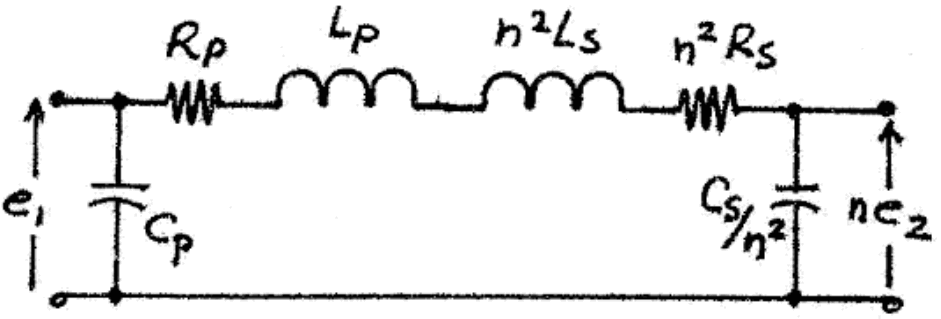
\includegraphics[width=0.32\linewidth]{_fig/potencia_modelo-transformador-c.png}
		\label{fig:potencia_modelo-transformador-c}
	}
	\caption{Modelos del Transformador}
	\label{fig:potencia_modelo-transformador}
\end{figure}

Es de hacer notar que este circuito representa un sistema de segundo orden, que podría conllevar a un pico de resonancia en la respuesta de frecuencia, la Figura \ref{fig:potencia_modelo-transformador-c}).

La configuración EC acoplado por transformador se plantea en la Figura \ref{fig:potencia_modelo-ec-acoplado-transformador}, junto con la recta de carga en continua y en alterna. 

\begin{figure}[h]
	\centering
	\subfloat[Esquema]
	{
		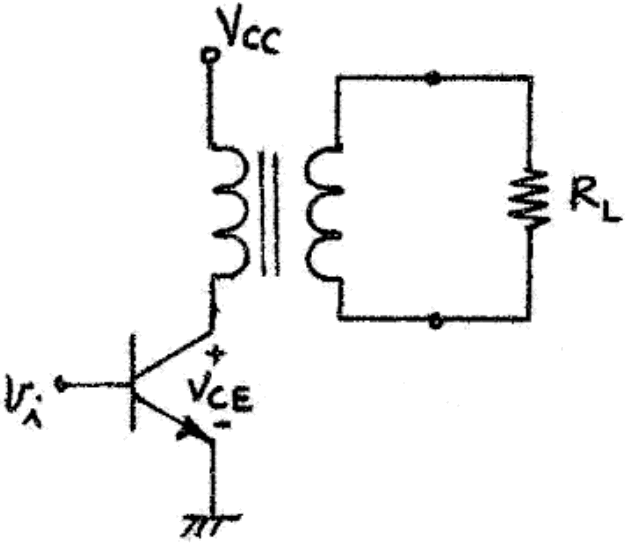
\includegraphics[width=0.44\linewidth]{_fig/potencia_modelo-ec-acoplado-transformador_esquema.png}
		\label{fig:potencia_modelo-ec-acoplado-transformador_esquema}
	}
	\subfloat[Rectas de carga]
	{
		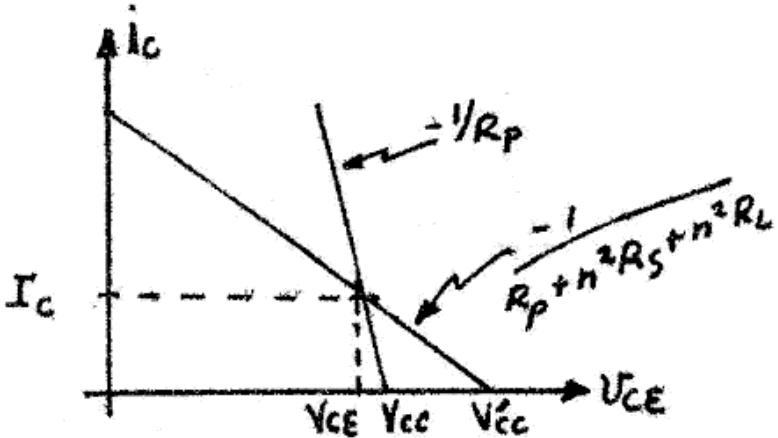
\includegraphics[width=0.44\linewidth]{_fig/potencia_modelo-ec-acoplado-transformador_grafo.png}
		\label{fig:potencia_modelo-ec-acoplado-transformador_grafo}
	}
	\caption{Configuracion EC acoplado por transformador}
	\label{fig:potencia_modelo-ec-acoplado-transformador}
\end{figure}

Se hace notar que la recta de carga en alterna tiene \underline{menos} pendiente que la recta de carga en continua, debido al acoplamiento de la resistencia de carga.

Se suponen condiciones ideales para calcular el rendimiento máximo óptimo ideal de este circuito; entonces \( V_{CE(\text{sat})} = 0 \), \( I_C(\text{corte}) = 0 \). Además, se desprecia \( R_p \) y \( R_s \), es decir, \( R_p, R_s = 0 \).

Resulta \( V_{CE} = V_{CC} \) y para lograr la recta de carga óptima en alterna se escoge \( n \) de modo que \( n^2 R_L I_C = V_{CE} \).

Queda: \( P_{CC} = I_C V_{CC} \)

y \( P_{\text{sal}}(\text{max}) = \frac{V_p I_p}{2} = \frac{V_{CE} I_C}{2} = \frac{V_{CC} I_C}{2} \)

Entonces \( \eta(\text{ideal}) = \frac{P_{\text{sal}}(\text{max})}{P_{CC}} = \frac{(V_{CC} I_C / 2)}{V_{CC} I_C} = \frac{1}{2} \)

Con un transformador se puede aspirar a conseguir un rendimiento máximo del 50\%, lo cual se compara favorablemente con un rendimiento máximo del 25\% para el circuito de la Figura 6.3. La mejora se debe a que no se desperdicia potencia de c.c. en la resistencia de carga. En condiciones de reposo la fuente de poder disipa potencia y el transistor disipa una potencia \( P_p = P_{CC} \).

Al aplicar señal, se reduce la disipación en el transistor en la misma proporción que se disipa potencia útil en la carga.

\section{Amplificadores Clase B} %p249

Para mejorar aún más el rendimiento de los amplificadores de potencia se utiliza el Amplificador Clase B. Existe una clasificación de los amplificadores basada en la fracción de la señal de entrada que es amplificada.

\begin{figure}[h]
	\centering
	\subfloat[Clase A]
	{
		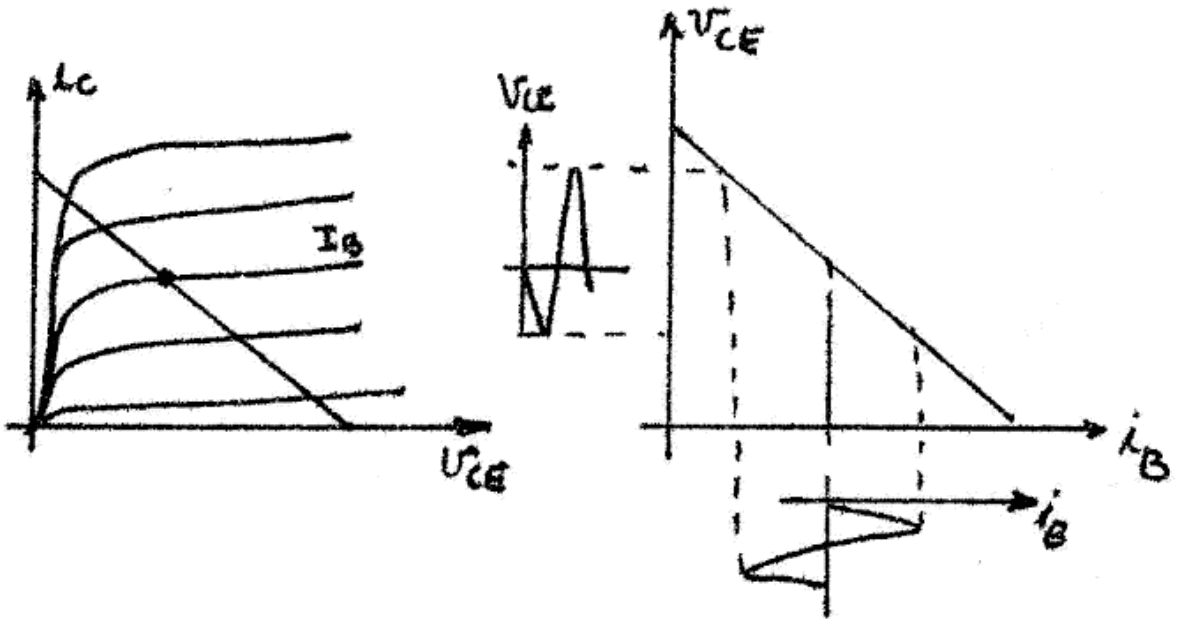
\includegraphics[width=0.22\linewidth]{_fig/potencia_caracteristica-clase-a.png}
		\label{fig:potencia_caracteristica-clase-a}
	}
	\subfloat[Clase B]
	{
		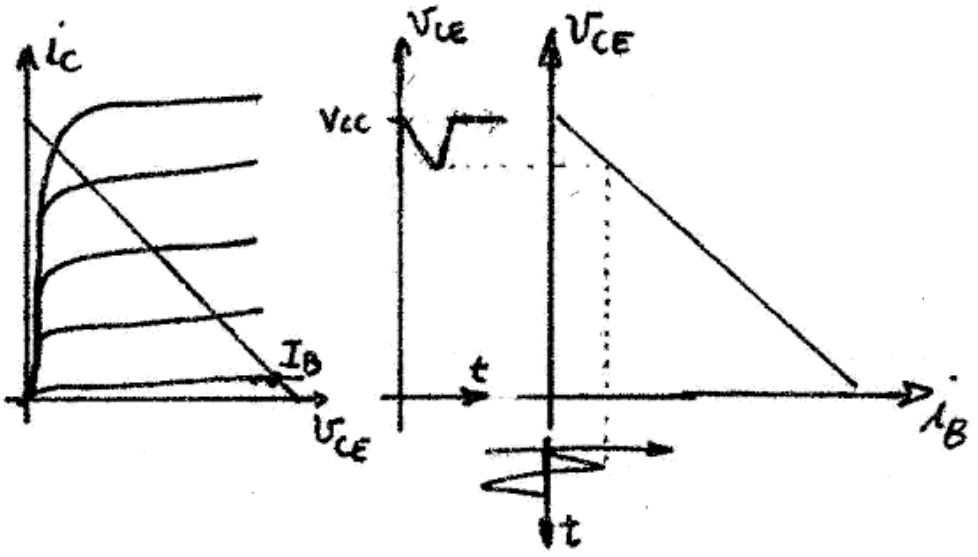
\includegraphics[width=0.22\linewidth]{_fig/potencia_caracteristica-clase-b.png}
		\label{fig:potencia_caracteristica-clase-b}
	}
	\subfloat[Clase C]
	{
		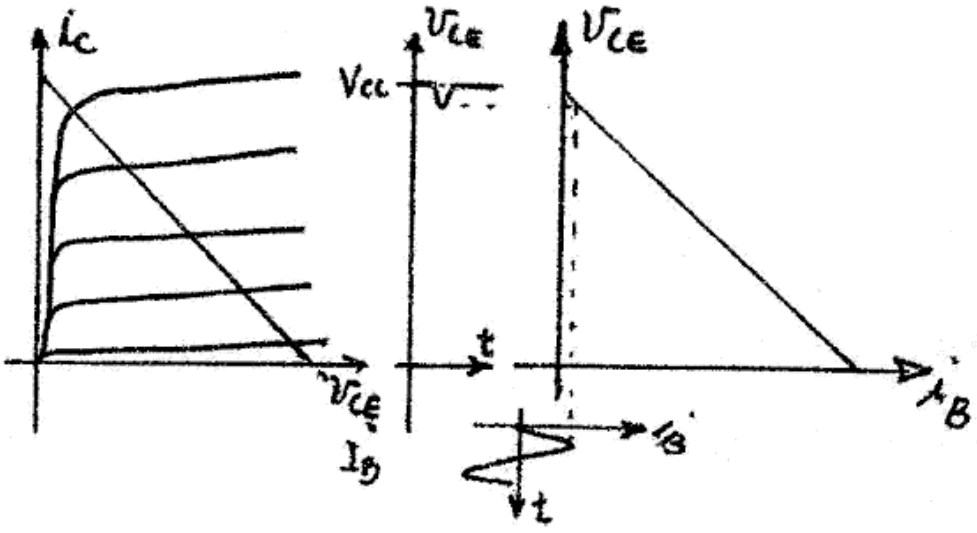
\includegraphics[width=0.22\linewidth]{_fig/potencia_caracteristica-clase-c.png}
		\label{fig:potencia_caracteristica-clase-c}
	}
	\subfloat[Clase D]
	{
		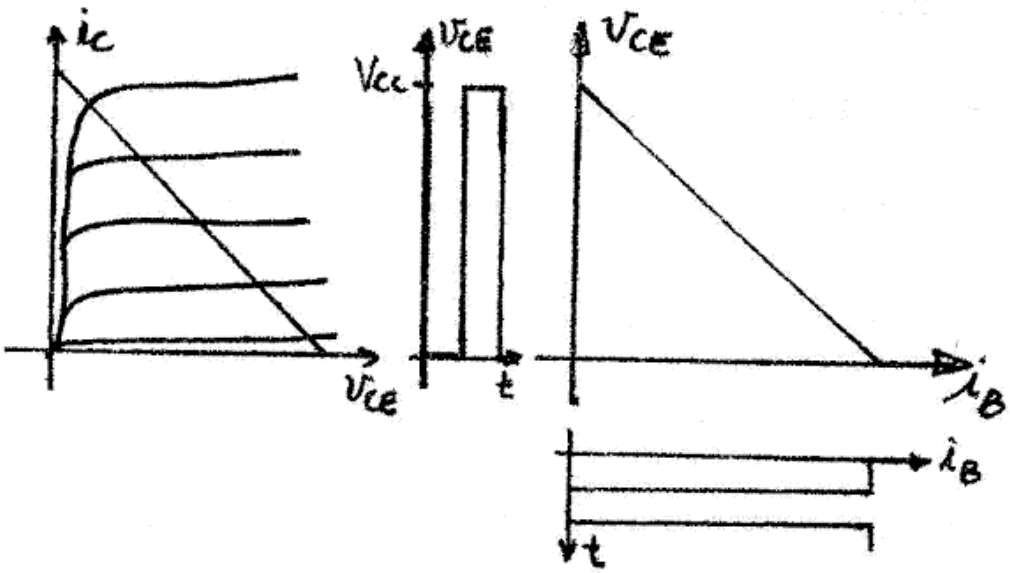
\includegraphics[width=0.22\linewidth]{_fig/potencia_caracteristica-clase-d.png}
		\label{fig:potencia_caracteristica-clase-d}
	}
	\caption{Modelos del Transformador}
	\label{fig:potencia_caracteristica-clase}
\end{figure}

Hasta ahora, los amplificadores han trabajado de modo que se amplifica la señal durante el ciclo completo. Esto corresponde al amplificador Clase A (ver Figura \ref{fig:potencia_caracteristica-clase-a}).

En el amplificador Clase B se amplifica la señal durante sólo medio ciclo (ver figura \ref{fig:potencia_caracteristica-clase-b}). En este caso, el transistor está polarizado al borde de corte o al borde de saturación.

En el amplificador Clase C se amplifica la señal durante menos de medio ciclo (ver Figura \ref{fig:potencia_caracteristica-clase-c}). Esto implica un punto de operación más allá del borde de corte para el NPN, $V_{BE}$ negativo.

La operación Clase D implica el funcionamiento del dispositivo entre los extremos de ON y OFF (por ejemplo, la compuerta CMOS), ver Figura \ref{fig:potencia_caracteristica-clase-d}.

En los amplificadores Clase B a transistores, se utilizan dos transistores, uno para el ciclo positivo de la señal y otro para el ciclo negativo; ver, por ejemplo, el circuito de la Figura \ref{fig:multietapas_etapa-salida_polarizacion} o la etapa de salida del 741, la Figura \ref{fig:multietapas_estructura-interna-ic_ua741}, formado por Q14 y Q16. Esta configuración presenta varias ventajas para los amplificadores de potencia: 

\begin{enumerate}
	\item En condiciones de reposo, la disipación de potencia es despreciable.
	\item El rendimiento es mayor que para los amplificadores Clase A; implícito en la segunda ventaja es el hecho que para cierta potencia de salida la fuente de poder es más pequeña; a la vez las exigencias de capacidad de disipación de potencia de los transistores son menores.
\end{enumerate}

Para mayor facilidad se vuelve a dibujar la configuración de simetría complementaria en la Figura \ref{fig:potencia_clase-b_simetria-complementaria}, la cual trabaja como un Amplificador Clase B. En condiciones de reposo, los transistores están polarizados al borde de corte, e $i_C = 0$.

\begin{figure}[h]
	\centering
	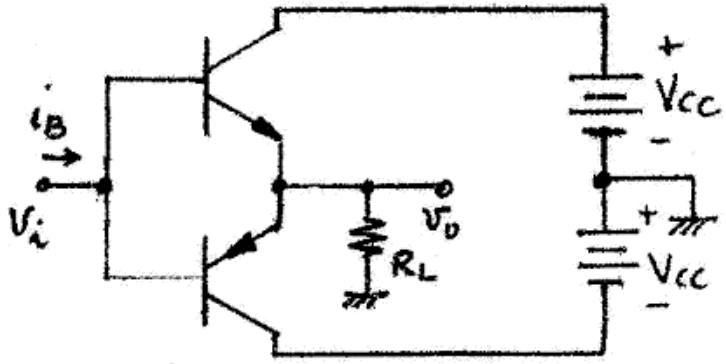
\includegraphics[width=0.8\linewidth]{_fig/potencia_clase-b_simetria-complementaria.png}
	\caption{Clase B: Simetria Complementaria}
	\label{fig:potencia_clase-b_simetria-complementaria}
\end{figure}

El punto de operación, la recta de carga y la característica de transferencia $i_{C1}$ vs $i_B$ se muestran en la Figura \ref{fig:potencia_clase-b_recta-de-carga}.

\begin{figure}[h]
	\centering
	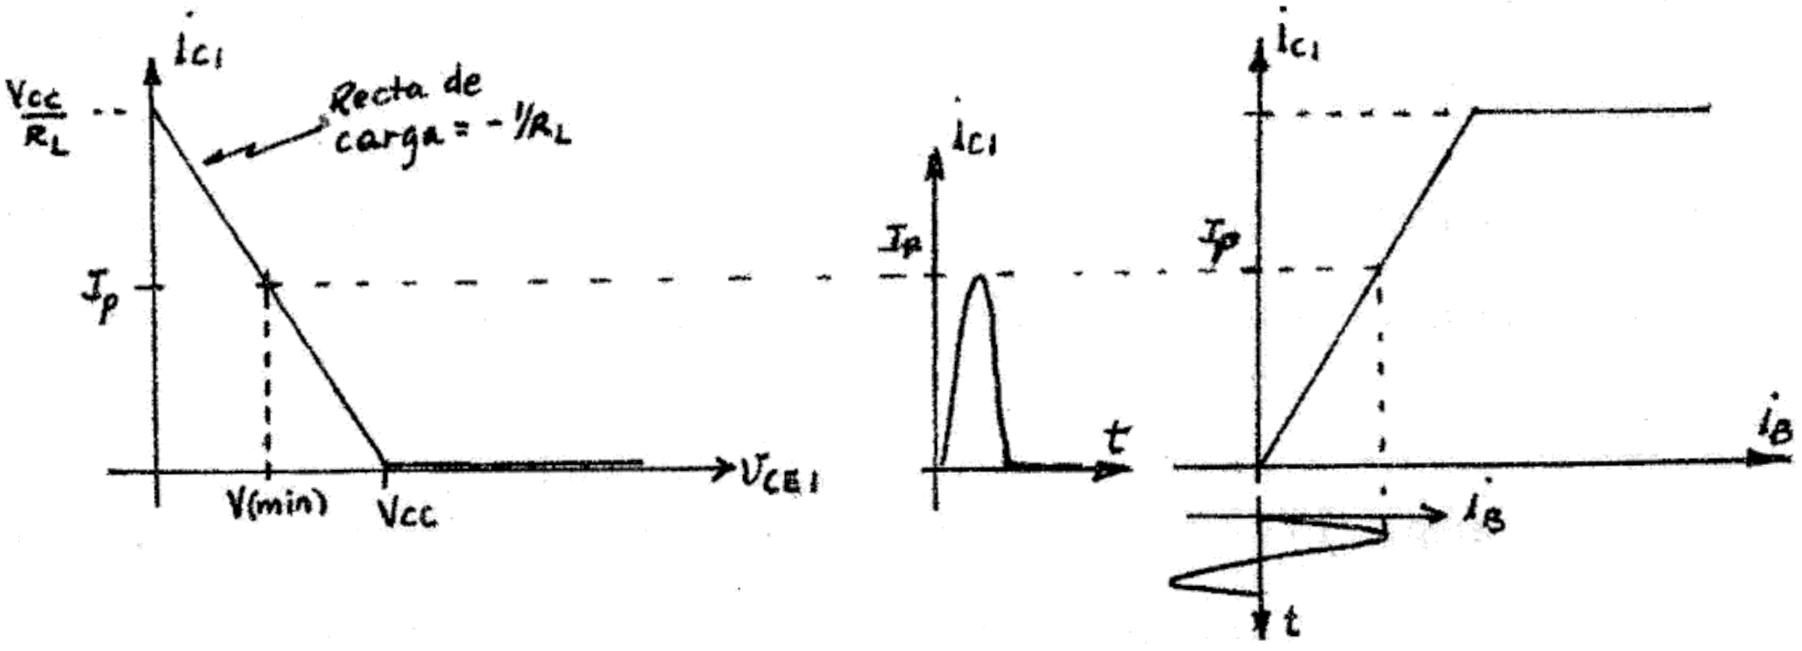
\includegraphics[width=0.8\linewidth]{_fig/potencia_clase-b_recta-de-carga.png}
	\caption{Clase B: Resta de Carga}
	\label{fig:potencia_clase-b_recta-de-carga}
\end{figure}

Al haber una variación positiva de la señal de entrada, aumenta la corriente de colector $i_{C1}$. Para señales negativas de entrada, entonces aumenta $|i_{C2}|$ mientras $i_{C1}$ permanece igual a 0. Entonces:

\begin{equation}
	i_{C1} = 
	\begin{cases}
		I_p \sin(\omega t) & 0 < t \leq T/2 \\
		0 & T/2 < t \leq T
	\end{cases}
\end{equation}

Esto implica un valor promedio (de continua) dado por:

\begin{equation}
	I_{C1} = \frac{1}{T} \int_0^T i \, dt = \frac{1}{T} \int_0^{T/2} I_p \sin(\omega t) \, dt = \frac{I_p}{\pi}
\end{equation}

La potencia entregada por la fuente positiva será:

\begin{equation}
	P_{cc}^{+} = I_{CC1} V_{CC} = I_P V_{CC} / \pi
\end{equation}

La potencia entregada por la fuente negativa será idéntica (para una señal de entrada simétrica), de donde la potencia entregada por las fuentes viene dada por:

\begin{equation}
	P_{cc} = P_{cc}^{+} + P_{cc}^{-} = 2 I_P V_{CC} / \pi
\end{equation}

La potencia de salida viene dada por:

\begin{equation}
	P_{sal} = \frac{I_{\text{ef}}^2 R}{2} = \frac{I_P^2 R_L}{2}
\end{equation}

y el rendimiento es:

\begin{equation}
	\eta = \frac{P_{sal}}{P_{cc}} = \frac{I_P R_L \pi}{4 V_{CC}}
\end{equation}

El máximo de $I_P$ es cuando hay máxima variación de $i_C$, es decir $i_C = V_{CC} / R_L$, de donde la máxima potencia de salida es:

\begin{equation}
	P_{sal}(\text{max}) = \frac{V_{CC}^2}{2 R_L}
\end{equation}

y el rendimiento máximo ideal es:

\begin{equation}
	\eta (\text{ideal}) = \frac{\pi}{4} \quad \text{(es decir el 78.5\%)}
\end{equation}

Esto es mucho mejor que el rendimiento máximo ideal del 50\% para amplificadores Clase A, y se consigue sin la necesidad de utilizar un transformador. Además, la potencia entregada por la fuente es cero en condiciones de reposo.

La potencia disipada en los transistores viene dada por:

\begin{equation}
	P_D = P_{cc} - P_{sal} = \frac{2 I_P V_{CC}}{\pi} - \frac{I_P^2 R_L}{2}
\end{equation}

Para hallar la máxima potencia disipada, efectuamos la derivada con respecto a $I_P$ y lo hacemos igual a cero:

\[
\frac{d P_D}{d I_P} = \frac{2 V_{CC}}{\pi} - I_P R_L = 0 \Rightarrow I_P = \frac{2 V_{CC}}{\pi R_L}
\]

Si convertimos este resultado en su equivalente de voltaje,

\[
V_{CE}(\text{min}) = V_{CC} - I_P R_L \Rightarrow V_{CE}(\text{min}) = V_{CC} - \frac{2 V_{CC}}{\pi} \approx 0.36 V_{CC}
\]

Para este valor de $V_{CE}(\text{min})$ la potencia disipada es máxima, y reemplazando en la ecuación (6.20) se consigue:

\begin{equation} \label{eq:potencia_p-disipada-maxima}
	P_D(\text{max}) = \frac{2}{\pi^2} \frac{V_{CC}^2}{R_L} = \frac{4}{\pi^2} P_{\text{sal}}(\text{max})
\end{equation}

Es decir $P_D(\text{max}) \approx 0.4\, P_{\text{sal}}(\text{max})$ o $\approx 0.314\, P_{CC}(\text{max})$

Es decir, si la fuente de poder entrega $10W$, se puede conseguir una potencia de salida máxima de $7.85W$, en donde $V_{CE}(\text{min}) = 0$, y bajo otra condición de $V_{CE}(\text{min}) = 0.36\,V_{CC}$, la potencia máxima disipada en los transistores es $3.14W$. Cuando se dice disipar $3.14W$ en los transistores, esto implica que se disipa $1.57W$ en cada transistor.

\section{La distorsión armónica} %p254

En un sistema lineal, la salida es una función linealmente proporcional a la entrada. Esto implica que en la salida no existen componentes de frecuencia que no existen en la entrada. Sin embargo, para variaciones grandes de señal, el transistor no trabaja en forma lineal; esto crea en la salida componentes de frecuencia no existentes en la entrada, y por lo tanto no deseables. Dado que las componentes creadas son armónicas (múltiples enteros) de la frecuencia de entrada, este defecto se denomina la distorsión armónica.

De la Figura \ref{fig:potencia_amplificador-ec_senal-grande}, se puede levantar una característica de transferencia que relaciona la corriente de entrada, $i_B$, con la corriente de salida, $i_c$, tal como se muestra en la Figura \ref{fig:potencia_distorcion_caracteristica-de-transferencia}.

\begin{figure}[h]
	\centering
	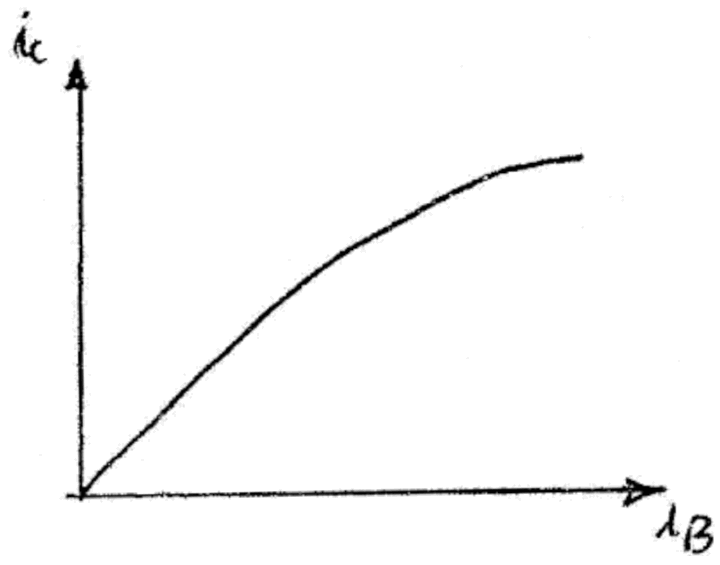
\includegraphics[width=0.8\linewidth]{_fig/potencia_distorcion_caracteristica-de-transferencia.png}
	\caption{Característica de transferencia, $i_B$ vs $i_C$}
	\label{fig:potencia_distorcion_caracteristica-de-transferencia}
\end{figure}

Para variaciones pequeñas de entrada se plantea la relación lineal:

\begin{equation} \label{eq:potencia_ic-variaciones-pequenas}
	I_c = \beta I_b + (\beta + 1) I_{c0} = G i_b + K
\end{equation}

Ahora para variaciones grandes de la entrada, una relación de segundo orden sería:

\begin{equation}
	i_c = G_1 i_b + G_2 i_b^2 + K
\end{equation}

Si $i_b = B_n \cos \omega t$, entonces:

\[
i_c = G_1 B_n \cos \omega t + G_2 B_n^2 \cos^2 \omega t + K
\]

\[
i_c = G_1 B_n \cos \omega t + \frac{G_2 B_n^2}{2} \cos 2\omega t + \frac{G_2 B_n^2}{2} + K
\]

\[
i_c = B_0 + B_1 \cos \omega t + B_2 \cos 2 \omega t
\]

De la expresión anterior se destaca que en la salida, $i_c$, aparece una componente a la frecuencia $2\omega$, es decir una frecuencia que no existe en la entrada.

Se puede obtener los valores de las componentes armónicas a través de varios aparatos como por ejemplo, un Analizador de Distorsión o un Analizador de espectro.

También se puede obtener una aproximación de las componentes armónicas en forma gráfica, de la característica de salida del transistor, la Figura \ref{fig:potencia_distorcion_caracteristica-de-salida}. El punto de operación Q representa las corrientes de base, $I_B'$, y de colector, $I_C'$, en continua.

\begin{figure}[h]
	\centering
	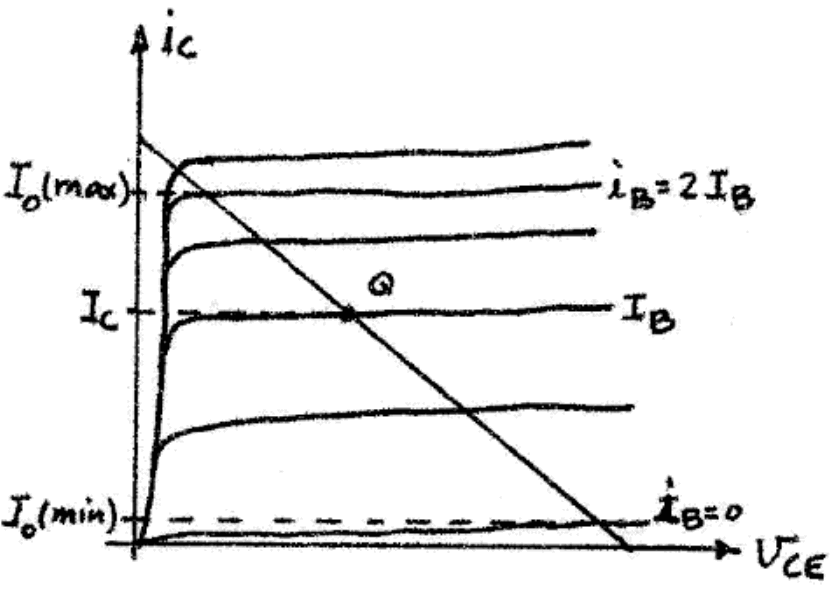
\includegraphics[width=0.8\linewidth]{_fig/potencia_distorcion_caracteristica-de-salida.png}
	\caption{Característica de Salida}
	\label{fig:potencia_distorcion_caracteristica-de-salida}
\end{figure}

Para una variación simétrica de la corriente de base, esta corriente alcanza un valor máximo de $2 I_B'$, para la cual $i_c = I_c(\text{max})$, y una corriente mínima de $I_B' = 0$, para la cual $i_c = I_c(\text{min})$.

La corriente de colector total es:

\[
i_c = i_c + I_C \text{, dado} i_b = I_B' + I_B \cos \omega t
\]

se tiene:

\begin{equation} \label{eq:potencia_i-colector}
	i_c = I_C + B_0 + B_1 \cos \omega t + B_2 \cos 2 \omega t
\end{equation}

Se puede encontrar $B_0$, $B_1$ y $B_2$ evaluando la Ecuación \ref{eq:potencia_i-colector} en tres puntos:

\begin{enumerate}
	\item[a)] Para $\omega t = 0$, $i_g$ e $i_c$ son máximos:
	\begin{equation} \label{eq:potencia_b0}
		I_o(\text{max}) = I_c + B_0 + B_1 + B_2
	\end{equation}
	
	\item[b)] Para $\omega t = \pi/2$, $i_g = I_g$ e $I_c$:
	\begin{equation} \label{eq:potencia_b1}
		I_c = I_c + B_0 - B_2
	\end{equation}
	
	\item[c)] Para $\omega t = \pi$, $i_g$ e $i_c$ son mínimos:
	\begin{equation} \label{eq:potencia_b2}
		I_o(\text{min}) = I_c + B_0 - B_1 + B_2
	\end{equation}
\end{enumerate}

De aquí que:

\begin{equation}
	B_0 = B_2 = \frac{I_o(\text{max}) + I_o(\text{min})}{4} - \frac{I_c}{2}
\end{equation}

\begin{equation}
	B_1 = \frac{I_o(\text{max}) - I_o(\text{min})}{2}
\end{equation}

La distorsión de la segunda armónica, $D_2$, viene dada por:

\begin{equation} \label{eq:potencia_da-2nd}
	D_2 = \frac{\text{componente 2a armónica}}{\text{componente fundamental}}
\end{equation}

Pueden (y suelen) existir componentes de las armónicas superiores, la 3a, 4ta, etc.; se procede en forma semejante a la correspondiente a las ecuaciones \ref{eq:potencia_i-colector} \ref{eq:potencia_b0} y \ref{eq:potencia_b1}, planteando tantas ecuaciones como incógnitas existan.

Después se puede calcular la distorsión de la armónica $n$: \( D_n = \frac{B_N}{B_1} \)

y la distorsión armónica total viene dada por:

\begin{equation} \label{eq:potencia_da}
	D = \sqrt{D_2^2 + D_3^2 + D_4^2 + \cdots}
\end{equation}

\subsection{Ejemplo}

En la Figura \ref{fig:potencia_amplificador-potencia_circuito} se plantea un amplificador de potencia y en la Figura \ref{fig:potencia_amplificador-potencia_caracteristica} la característica de salida para el transistor utilizado.

\begin{figure}[h]
	\centering
	\subfloat[Circuito]
	{
		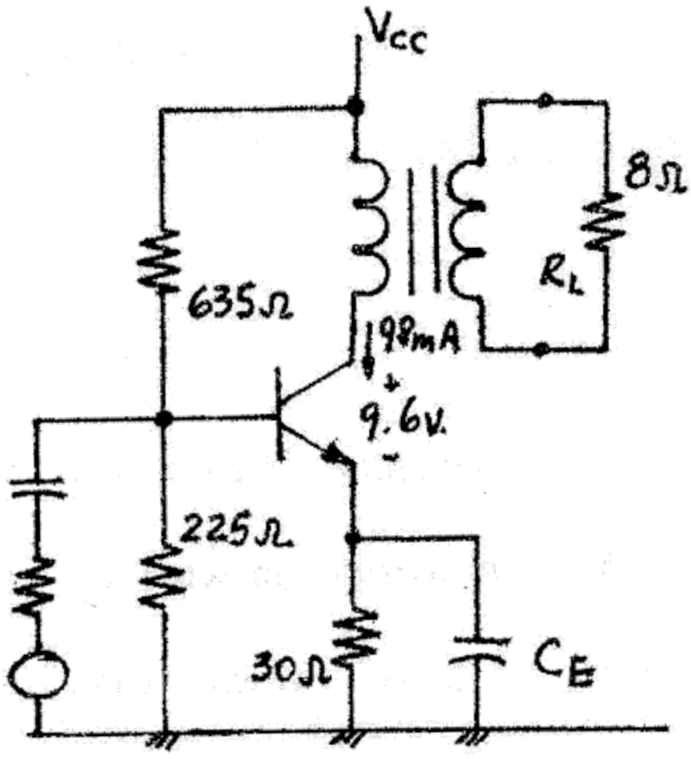
\includegraphics[width=0.3\linewidth]{_fig/potencia_amplificador-potencia_circuito.png}
		\label{fig:potencia_amplificador-potencia_circuito}
	}
	\subfloat[Característica y Recta para el Transistor]
	{
		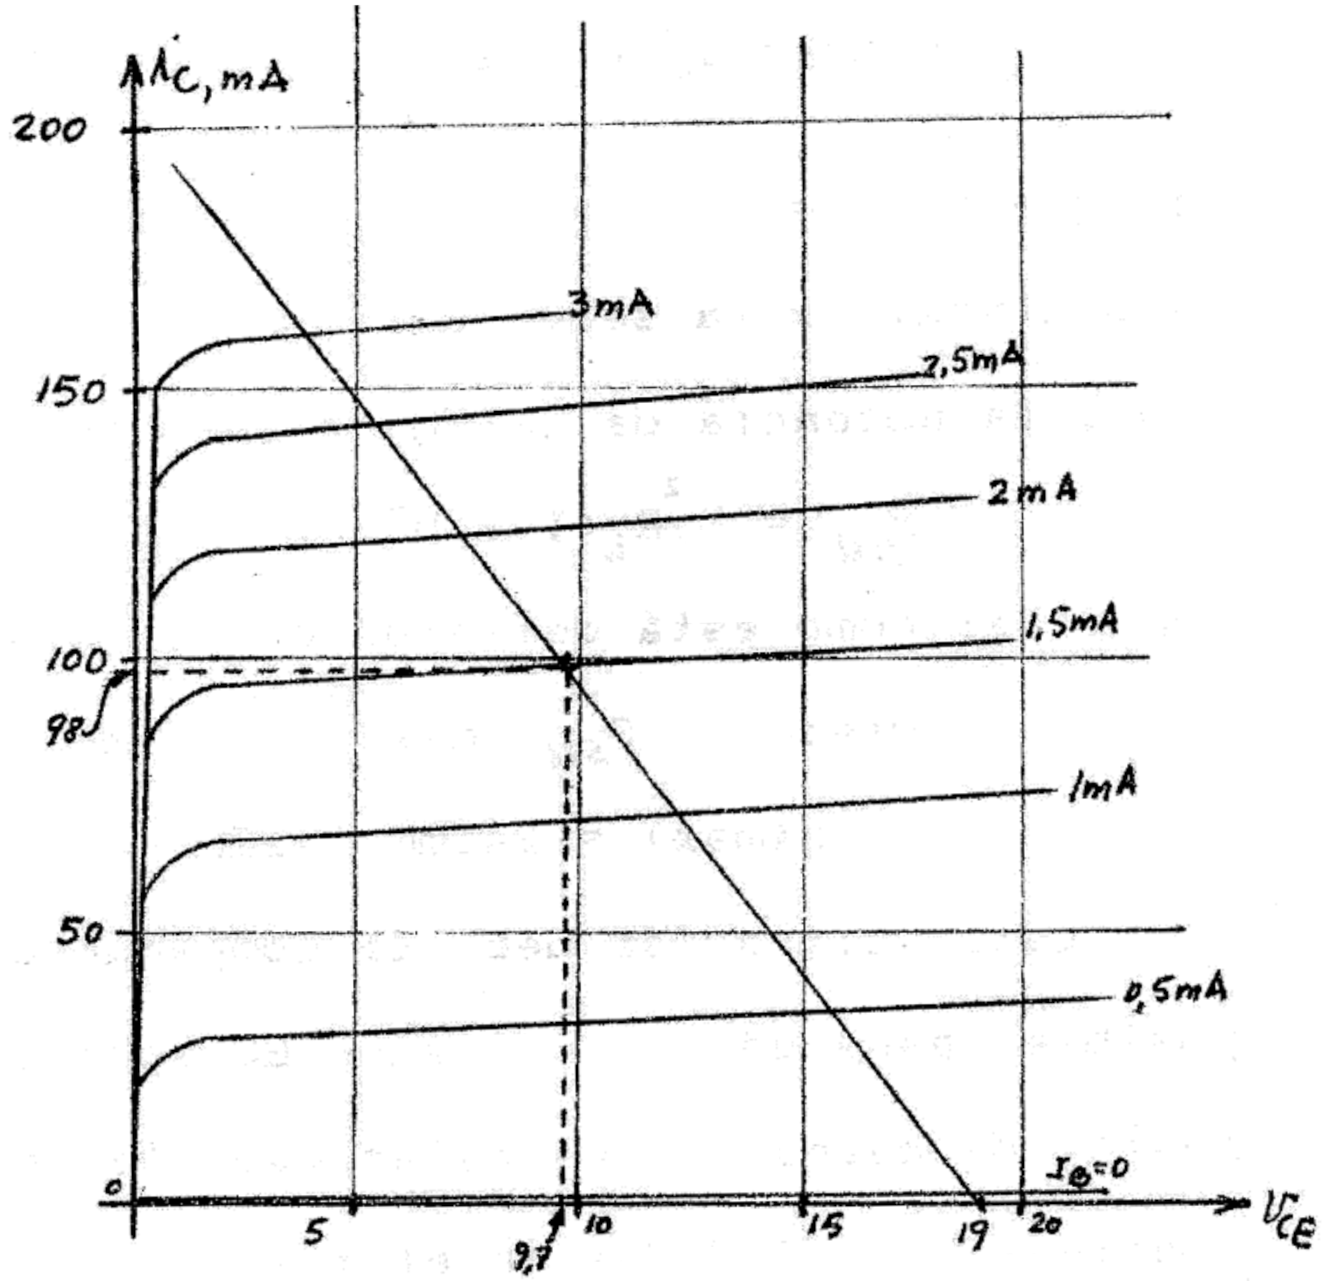
\includegraphics[width=0.66\linewidth]{_fig/potencia_amplificador-potencia_caracteristica.png}
		\label{fig:potencia_amplificador-potencia_caracteristica}
	}
	\caption{Amplificador de Potencia}
	\label{fig:potencia_amplificador-potencia}
\end{figure}

Para el transformador se tiene que $R_P = 8\Omega$, $R_S = 1\Omega$, $n = 3.12$.

Se ha fijado el punto de operación en $(I_B, I_C, V_{CE}) = (1.5\,\text{mA},\ 98\,\text{mA},\ 9.6\,\text{V})$, de donde el valor de la fuente viene dado por:

\[
V_{CC} = I_C R_P + V_{CE} + I_E R_E = 13.6\,\text{V}
\]

En corriente alterna, el condensador $C_E$ puentea la resistencia del emisor y la resistencia que queda en la malla de salida es igual a: \( R_P + n^2 R_S + n^2 R_L = 95.8 \Omega\); con este valor se traza la recta de carga de C.A. La corriente de base variará entre $0 mA$ y $3 mA$; los valores para la corriente de colector son $4.5 mA$ y $162 mA$ respectivamente. 

De las ecuaciones \ref{eq:potencia_p-disipada-maxima} y \ref{eq:potencia_ic-variaciones-pequenas} se consigue:

\[
B_0 = B_2 = -8.3 \text{mA}
B_1 = 78.8 \text{mA}
\]

de donde la distorsión de la segunda armónica:

\[
D_2 = \left| \frac{B_2}{B_1} \right| = 10.5\%
\]

El valor de $D_2 = 10.5\%$ es generalmente malo. Una distorsión que puede calificarse de baja en los amplificadores comerciales está por el orden del $1\%$ o menos. Otro resultado interesante es que la corriente que suministra la fuente de poder disminuye con señal por un valor de $B = -8.3\,\text{mA}$; esto se debe nuevamente al funcionamiento no lineal del transistor.

Se puede encontrar el rendimiento máximo (no necesariamente óptimo) para este circuito bajo condiciones de la variación máxima simétrica de la señal de entrada:

\[
P_{CC} = V_{CC} I_C' = 13.6 (I_C + B_0) = 13.6 \text{V} (98 - 8.3) \text{mA} = 1.22 \text{W}
\]

\[
P_{sal}(\text{máx}) = \frac{I_P^{\prime 2} R_L^{\prime}}{2} = \frac{(78.8\,\text{mA} + 8.3\,\text{mA})^2 \times (3.12)^2 \times 8}{2}
\]

ya que $R_L^{\prime} = n^2 8\,\Omega$ y las componentes de alterna consisten de la fundamental y la segunda armónica. En la presencia de distorsión, la potencia de salida viene dada por:

\begin{equation}
	P_{sal} = B_1^2 R_L^{\prime} (1 + D_2^2)/2
\end{equation}

con $D$ tal como está definido en la ecuaciones \ref{eq:potencia_da-2nd} y \ref{eq:potencia_da}.

Después:

\[
P_{sal}(\text{máx}) = 245\,\text{mW}
\]

y

\[
\eta(\text{máx}) = \frac{245\,\text{mW}}{1.22\,\text{W}} = 19.9\%
\]

Esta cifra se debe comparar con el máximo rendimiento posible para un amplificador EC acoplado por transformador.

El punto de operación es relativamente óptimo.  
Sin embargo, en continua hay pérdidas en el transformador y en la resistencia del emisor, y en alterna hay pérdidas en el transformador.

\section{Amplificadores de contrafase} %p259

En esta sección se muestra una forma de reducir la distorsión utilizando un amplificador en contrafase, como se ve en la Figura \ref{fig:potencia_amplificador-contrafase_circuito} con dos transistores \textit{NPN}.

\begin{figure}[h]
	\centering
	\subfloat[Circuito]
	{
		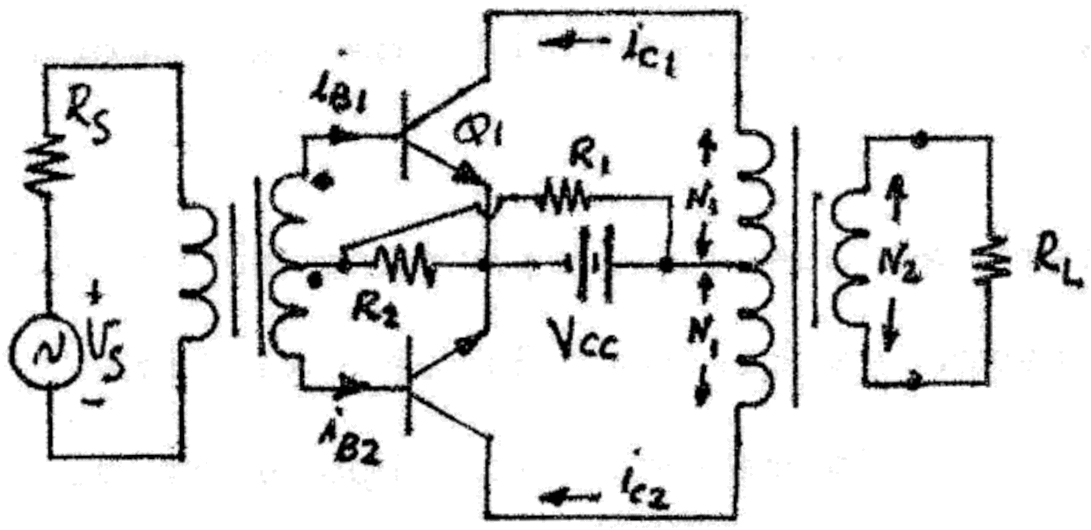
\includegraphics[width=0.6\linewidth]{_fig/potencia_amplificador-contrafase_circuito.png}
		\label{fig:potencia_amplificador-contrafase_circuito}
	}
	\subfloat[Disposición de las bobinas del transformador]
	{
		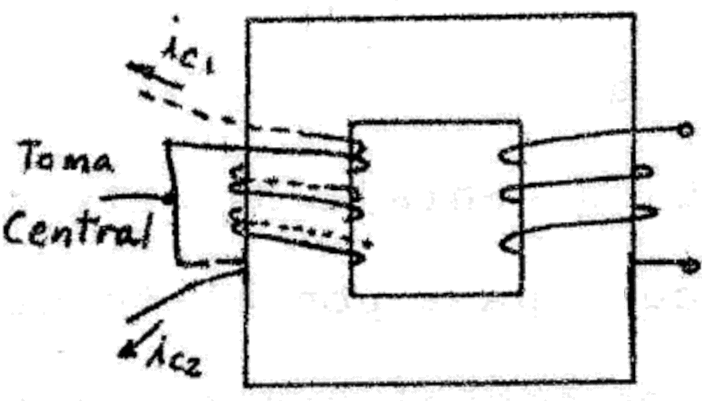
\includegraphics[width=0.3\linewidth]{_fig/potencia_amplificador-contrafase_disposicion.png}
		\label{fig:potencia_amplificador-contrafase_disposicion}
	}
	\caption{Amplificador en contrafase}
	\label{fig:potencia_amplificador-contrafase}
\end{figure}

El transformador a la entrada sirve como un inversor de fase, es decir, la señal de entrada a \( Q_2 \) será de igual magnitud pero de polaridad opuesta en relación a la señal de entrada de \( Q_1 \).

Por lo tanto, si
\begin{equation}
	i_{b1} = b_{1} + I_B = B_m \cos(\omega t) + I_B
\end{equation}

entonces
\begin{equation}
	i_{c1} = I_C + B_0 + B_1 \cos(\omega t) + B_2 \cos(2\omega t) + B_3 \cos(3\omega t) + \ldots
\end{equation}

y
\begin{equation}
	i_{b2} = I_C + i_{b2} = I_B - i_{b1} = I_B + B \cos(\omega t + \pi)
\end{equation}

de donde
\begin{equation}
	i_{c2} = I_C + B_0 + B_1 \cos(\omega t + \pi) + B_2 \cos(2(\omega t + \pi)) + B_3 \cos(3(\omega t + \pi)) + \ldots \\
	i_{c2} = I_C + B_0 - B_1 \cos(\omega t) + B_2 \cos(2\omega t) - B_3 \cos(3\omega t) + \ldots
\end{equation}

En el transformador de salida circula \( i_{c1} - i_{c2} \), tal como se aprecia en la Figura \ref{fig:potencia_amplificador-contrafase_disposicion}:

\begin{equation}
	i_{cl} - i_{c2} = 2\left(B_1 \cos(\omega t) + B_3 \cos(3\omega t) + \ldots\right)
\end{equation}

De donde se observa que se eliminan las armónicas pares, en particular la segunda, que puede ser la más notable. La resistencia de carga referida al primario tiene un valor igual a:

\[
2\left( \frac{N_1}{N_2} \right)^2 R_L
\]

En este desarrollo se ha supuesto que los transistores tienen características idénticas. En la práctica, esto difícilmente se logra, por lo que los coeficientes \( B_0 \), \( B_1 \), \( B_2 \), etc., de \( i_{c1} \) e \( i_{c2} \) no son idénticos y podrá aparecer distorsión de la segunda armónica.

Otra ventaja de este sistema es que la componente de continua que pasa por el transformador es cero. Si se analiza la curva de magnetización para un transformador, la Figura \ref{fig:potencia_amplificador-contrafase_curva-magnetizacion}, se hace notar que la característica se satura para corrientes grandes. 

\begin{figure}[h]
	\centering
	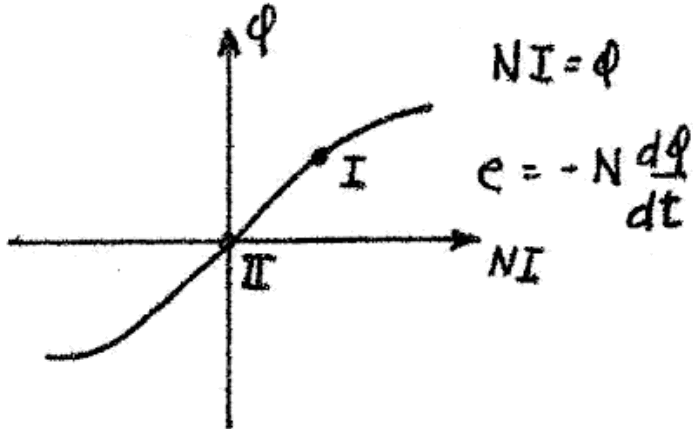
\includegraphics[width=0.8\linewidth]{_fig/potencia_amplificador-contrafase_curva-magnetizacion.png}
	\caption{Curva de Magnetización}
	\label{fig:potencia_amplificador-contrafase_curva-magnetizacion}
\end{figure}

Cuando circula una corriente continua por el transformador, como en el circuito de la Figura \ref{fig:potencia_modelo-ec-acoplado-transformador}, esto corresponde a un punto \( I \) de la característica, el cual se encuentra cercano al codo de la curva. La relación entre corriente y flujo no es lineal y se crea distorsión en la salida.

Para evitar este efecto se tendrá que utilizar un transformador más grande, que sea capaz de aguantar un flujo mayor. 

En cambio, si la corriente que circula por el transformador en continua es cero, como en el amplificador de contrafase, esto corresponde al punto \( II \) de la característica, y al estar en el medio de la curva, se aprovecha mejor el transformador.

\section{Reducción de distorsión con retroalimentación} %p261

En las secciones anteriores, se describió el fenómeno de la distorsión armónica: cómo surge, cómo calcularla y cómo reducirla.

Ahora se presenta una configuración retroalimentada que incorpora un preamplificador de ganancia elevada para reducir esta y otros tipos de distorsión, lo que representa una solución general y efectiva. 

Por ejemplo, surge distorsión si la fuente de alimentación DC tiene una regulación pobre, que se refleja en un rizado en la señal de salida. O en la configuración Clase B, vista anteriormente, que presenta una fuerte distorsión de cruce: cada vez que la señal \( v_i \) en la Figura \ref{fig:potencia_clase-b_simetria-complementaria} está entre \(-0.6 V\) y \(+0.6 V\), la salida es cero, como se destaca en la relación de transferencia de la Figura \ref{fig:potencia_reduccion-distorcion_relacion-transferencia}, con la consecuente relación de tiempo para un caso de señal sinusoidal que se muestra.

\begin{figure}[h]
	\centering
	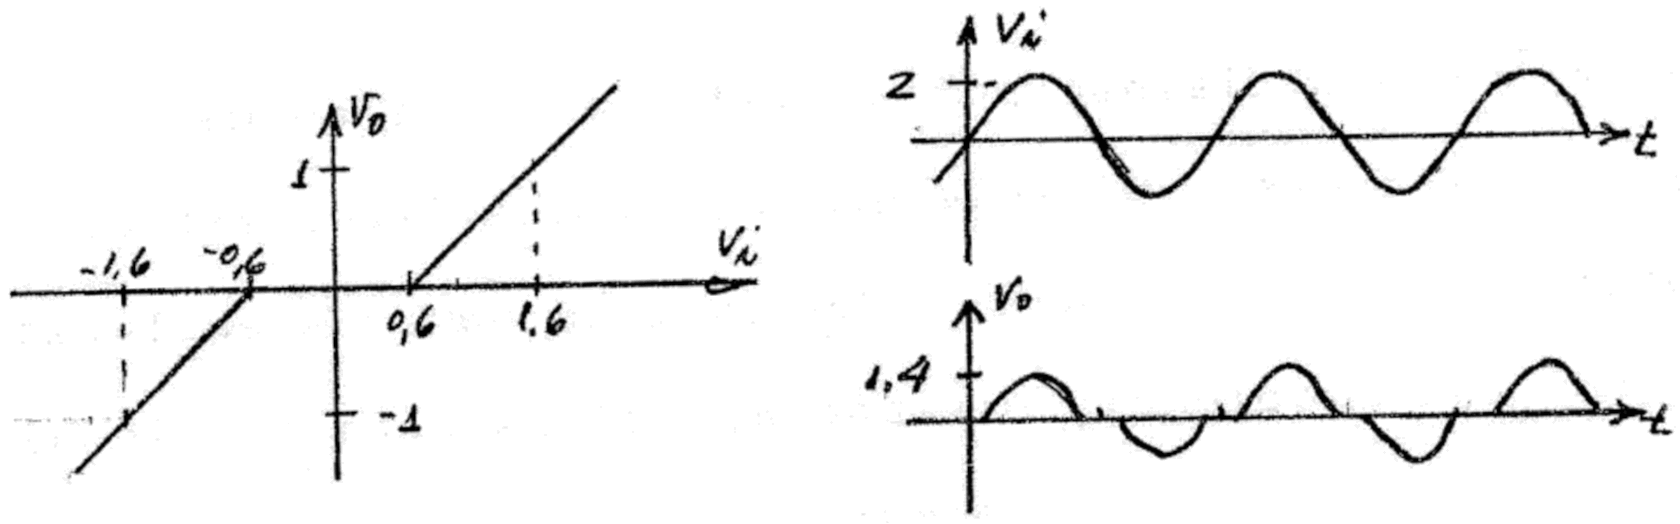
\includegraphics[width=0.8\linewidth]{_fig/potencia_reduccion-distorcion_relacion-transferencia.png}
	\caption{Reduccion de distorcion, relacion de transferencia}
	\label{fig:potencia_reduccion-distorcion_relacion-transferencia}
\end{figure}

Con la configuración de la Figura \ref{fig:potencia_reduccion-distorcion_circuito}, se reduce el voltaje umbral de la Figura \ref{fig:potencia_reduccion-distorcion_relacion-transferencia} por el factor \( 1 + A\beta \). Por ejemplo, si \( A = 10^6 \) y \( \beta = 1 \), el voltaje umbral de 0.6V se reduce a 6 $\mu$V, un nivel prácticamente despreciable. Para aplicaciones de audio con el 741 hay que tener en cuenta que \( A \) disminuye con la frecuencia. Por ejemplo, para \( f = 10 \, \text{kHz} \), \( A(f) \approx 100 \), y si \( \beta = \frac{1}{10} \), entonces el voltaje umbral se habrá reducido apenas a 60 mV, y la distorsión de cruce se hará notar nuevamente.

\begin{figure}[h]
	\centering
	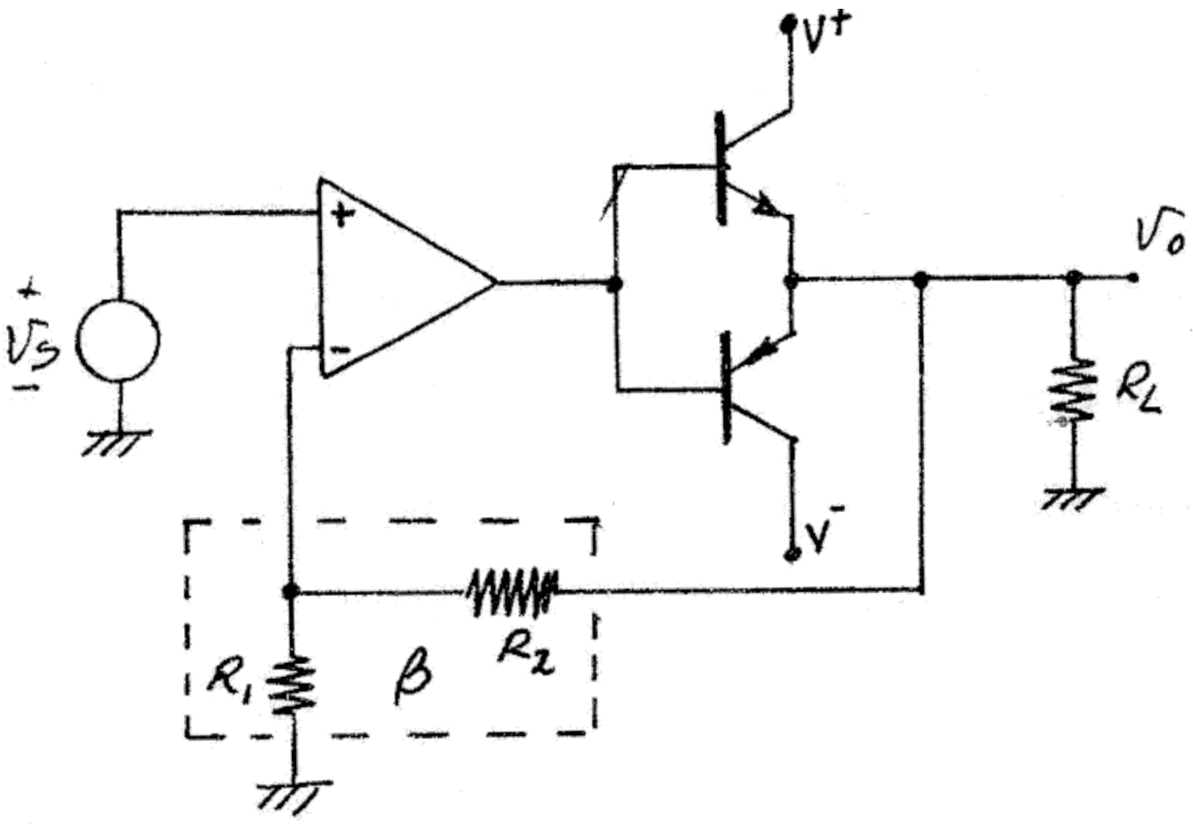
\includegraphics[width=0.8\linewidth]{_fig/potencia_reduccion-distorcion_circuito.png}
	\caption{Reduccion de distorcion, circuito}
	\label{fig:potencia_reduccion-distorcion_circuito}
\end{figure}

\section{Consideraciones térmicas} %p262

Dispositivos como transistores, diodos, triacs, reguladores, etc., que se utilizan en las etapas de potencia de un equipo van a disipar potencias relativamente elevadas y tienden a recalentarse. Si internamente los dispositivos exceden una temperatura límite se dañan. En esta sección vamos a analizar la relación entre potencia disipada y temperatura para el transistor, aunque los procedimientos son aplicables directamente a otros dispositivos.

Se comprueba experimentalmente la relación:

\begin{equation}
	T_a + \theta_t P_R = T_j
\end{equation}

donde:
\begin{itemize}
	\item \( T_a \) es la temperatura ambiental,
	\item \( \theta_t \) es la resistencia térmica,\\
	\item \( P_R \) es la potencia removida,
	\item \( T_j \) es la temperatura de juntura del transistor.
\end{itemize}

Cuanto más pequeña es la resistencia térmica, más fácilmente se disipa el calor generado por el dispositivo y menor será la diferencia entre \( T_a \) y \( T_j \).

En la Figura \ref{fig:potencia_p-t_transistor}.se indica la relación entre el valor de la máxima potencia removida y la temperatura para un dispositivo.

\begin{figure}[h]
	\centering
	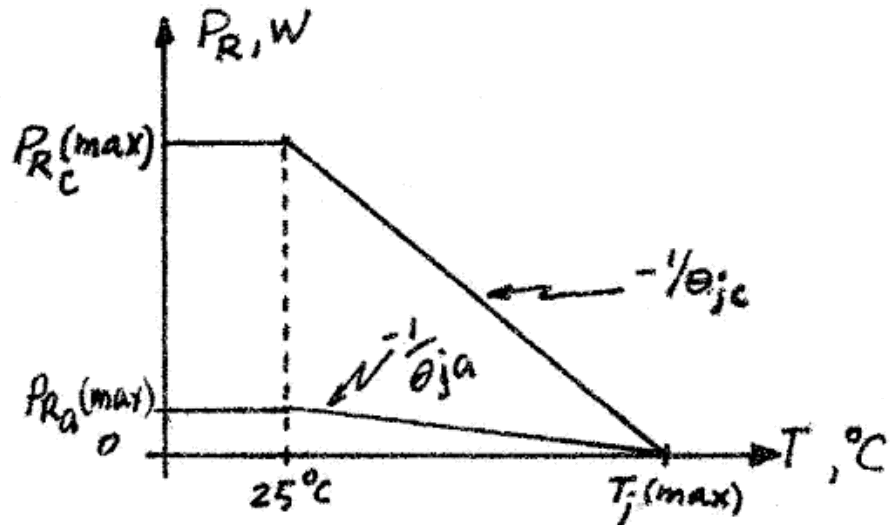
\includegraphics[width=0.8\linewidth]{_fig/potencia_p-t_transistor.png}
	\caption{$P$ vs $T$ para un transistor}
	\label{fig:potencia_p-t_transistor}
\end{figure}

Hay dos curvas:
\begin{itemize}
	\item La superior representa un sumidero térmico ideal (\(\theta = \infty\)) y la relación entre la potencia removida máxima \( P_{Rc} \) y la temperatura de la cubierta \( T_c \).
	\item La inferior considera el transistor sin sumidero térmico, con la potencia removida máxima \( P_{Ra(max)} \) y la temperatura ambiental \( T \).
\end{itemize}

Con un sumidero térmico, la potencia removida máxima \( P_{R(max)} \) es mayor que sin él. El valor de \( \theta \) es igual al inverso de la pendiente. A \( 25^\circ C \), se especifica el valor máximo seguro de potencia. También se indica la temperatura de juntura máxima: si la temperatura ambiental alcanzara este valor, cualquier potencia disipada en el transistor podría dañarlo. La relación entre la potenciam removida y la temperatura de la cubierta (o caja) del transistor obedece a la siguiente ecuación:

\begin{equation}
	T_c + \theta_c P_R = T_j
\end{equation}

Donde:
\begin{itemize}
	\item \(T_c\) es la temperatura de la cubierta del transistor.
	\item \(\theta_c\) es la resistencia térmica entre la cubierta y el sumidero térmico.
	\item \(P_R\) es la potencia disipada.
	\item \(T_j\) es la temperatura de la juntura del transistor.
\end{itemize}

Se establece que la resistencia térmica entre la juntura y la cubierta \(\theta_{jc}\) es menor que la resistencia térmica entre la juntura y el ambiente \(\theta_{ja}\), es decir, \( \theta_{jc} < \theta_{ja} \), y generalmente es mucho menor,  \( \theta_{jc} << \theta_{ja} \)

Además, cuando se utiliza un sumidero térmico, la resistencia térmica total se expresa como:

\[
\theta_T = \theta_{js} + \theta_{cs} + \theta_{sa}
\]

Donde:
\begin{itemize}
	\item \(\theta_{js}\) es la resistencia térmica entre la juntura y el sumidero.
	\item \(\theta_{cs}\) es la resistencia térmica entre la cubierta y el sumidero.
	\item \(\theta_{sa}\) es la resistencia térmica entre el sumidero y el ambiente, la cual puede ser muy pequeña si el simidero si el sumidero tiene las dimensiones grandes.
\end{itemize}

Una relación entre \(\theta\) y el tamaño del sumidero se muestra en la Figura \ref{fig:potencia_termica_placa-aluminio-3mm}. En resumen \(\theta_T\) será menor si se utiliza un sumidero para disipar el calor.

\begin{figure}[h]
	\centering
	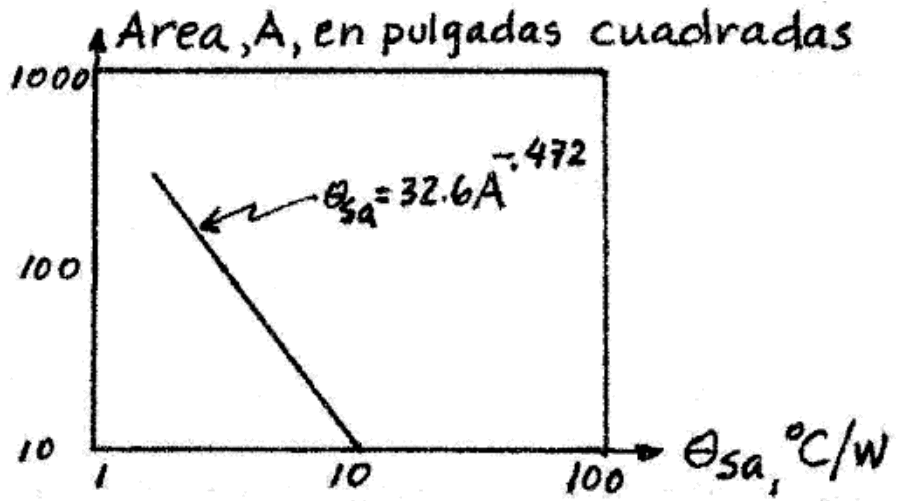
\includegraphics[width=0.8\linewidth]{_fig/potencia_termica_placa-aluminio-3mm.png}
	\caption{$\delta$ de una placa de alumino con $3\text{mm}$ de espesor}
	\label{fig:potencia_termica_placa-aluminio-3mm}
\end{figure}

\subsection{Ejemplo}
El transistor TIP36 tiene una \( \theta_{ja} = 35.7 \, °C/W \) y una relación entre \(P_R\) y temperatura de la cubierta que se muestra en la Figura \ref{fig:potencia_pr-tc-tip36}. Determine la máxima potencia disipada cuando se utiliza un sumidero térmico con superficie de área \(= 20 \text{in}^2\), suponer \( \theta_{cs} = 0.5 \frac{\circ C}{W} \)

\begin{figure}[h]
	\centering
	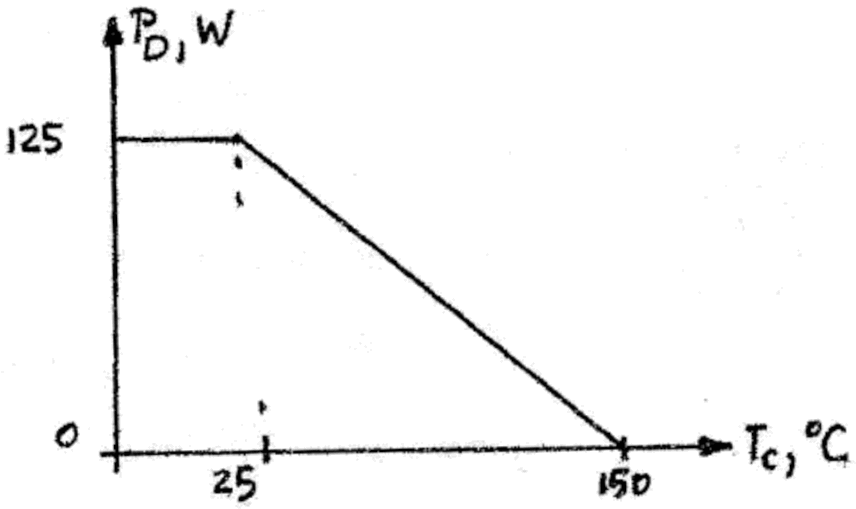
\includegraphics[width=0.8\linewidth]{_fig/potencia_pr-tc-tip36.png}
	\caption{$P_R$ vs $T_C$ para el TIP36}
	\label{fig:potencia_pr-tc-tip36}
\end{figure}

\textbf{Solución:}

De la figura \ref{fig:potencia_pr-tc-tip36} se tiene:

\[
T_C (25^\circ C) + P_R (25^\circ C) \theta_{jc} = T_C (150^\circ C) + P_R (150^\circ C) \theta_{jc}
\]

\[
25^\circ + 125 \theta_{jc} = 150^\circ + \theta
\]

\[
\theta_{jc} = \frac{(150^\circ - 25^\circ)}{125} = 1 \frac{C}{W}
\]

De la Figura \ref{fig:potencia_termica_placa-aluminio-3mm}, con un área de \(20 \text{in}^2\), se obtiene: \( \theta_{sa} = 8 \frac{C}{W} \). Entonces, con sumidero, se tiene:

\[
\theta_T = \theta_{jc} + \theta_{cs} + \theta_{sa} = (1 + 0.5 + 8) \frac{C}{W} = 9.5 \frac{C}{W}
\]

Se observa que \(\theta_T\) con sumidero térmico es menor que \(\theta_{ja}\) del transistor. A partir de la ecuación (6.31), la potencia máxima disipable es:

\[
P_{R(max)} = P(25) = \frac{(T_J(max) - 25^\circ)}{\theta_T} = \frac{125^\circ}{9.5 \frac{C}{W}} = 13.2 W
\]

Esto indica que, aunque el transistor puede disipar hasta 125 W con una temperatura de cubierta de \( 25^\circ C\), cuando se utiliza un sumidero térmico con \(\theta_{sa} = 8 \frac{C}{W}\), solo puede disipar \( 13.2 W\). En la Figura \ref{fig:potencia_temperatura-punto-interes-circuito}, se indica la temperatura en cada punto de interés del ejemplo anterior a través de un modelo basado en circuitos electricos con:

\begin{itemize}
	\item \( P \) (potencia) \(\rightarrow\) \( I \) (corriente)
	\item \( T \) (temperatura) \(\rightarrow\) \( V \) (tensión)
	\item \( \theta \) (resistencia térmica) \(\rightarrow\) \( R \) (resistencia)
\end{itemize}

\begin{figure}[h]
	\centering
	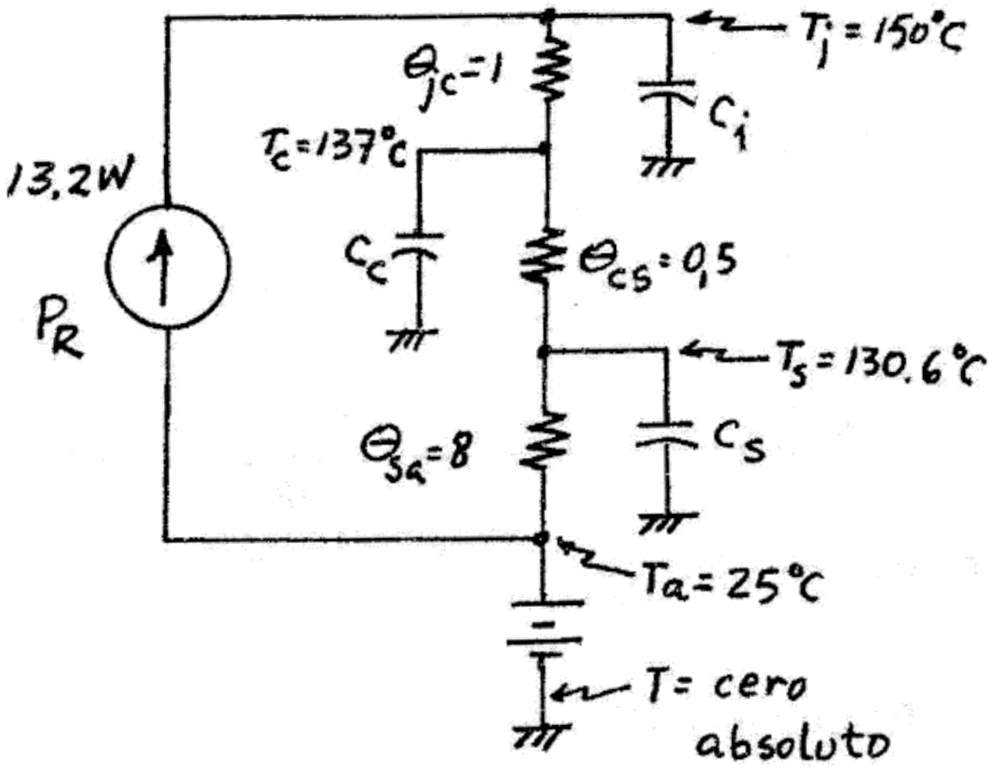
\includegraphics[width=0.8\linewidth]{_fig/potencia_temperatura-punto-interes-circuito.png}
	\caption{Temperatura en puntos de interes en un circuito}
	\label{fig:potencia_temperatura-punto-interes-circuito}
\end{figure}

Los condensadores modelan la inercia de los sistemas térmicos.

Finalmente hablemos del fenómeno conocido como \textit{corrimiento térmico}. Se puede dar el caso debido a un aumento de temperatura aumenta la potencia disipada que a su vez aumenta la temperatura, y asi entrar en un circulo vicioso, que termina por destruir el dispositivo. Para evitar esa espiral perjudicial, es necesario asegurar que se pueda remover mnayor potencia de la que se pueda generar debido a esos aumentos de temperatura, es decir:

\begin{equation}
	\frac{\partial P_G}{\partial T_J} < \frac{\partial P_R}{\partial T_J}
\end{equation}

De la ecuación 6.32, en condiciones ambientales:

\begin{equation}
	\frac{\partial P_R}{\partial T_J} = \frac{1}{\theta_{JT}}
\end{equation}

Además:

\begin{equation}
	\frac{\partial P_G}{\partial T_J} = \frac{\partial P_G}{\partial I_C} \cdot \frac{\partial I_C}{\partial T_J}
\end{equation}

Para una configuración en emisor común (EC), como la mostrada en la Figura 6.13, se obtiene:

\[
P_G = V_{CE} I_C = V_{CC} I_C - I_C^2 (R_C + R_E)
\]

De donde:

\[
\frac{\partial P_G}{\partial I_C} = V_{CC} - 2 I_C (R_C + R_E)
\]

además 

\[
\frac{\partial I_C}{\partial T_J} = S
\]

el factor de estabilidad en dispositivos de silicio se expresa como:

\[
\frac{\partial I_C}{\partial T_j} = 0.07 I_C
\]

Es decir, hay un aumento de \( 7\% \) por cada grado de incremento en la temperatura de juntura \( T_j \).

Por lo tanto, para el circuito de la Figura 6.13, la potencia disipada debe cumplir:

\begin{equation}
	\frac{\partial P_d}{\partial T_j} = \left[ V_{CC} - I_C (R_C + R_E) \right] \leq (0.07 I_C) \quad (6.37)
\end{equation}

y se tiene que cumplir la relación:

\begin{equation}
	\frac{\partial P_d}{\partial T_j} < \frac{1}{\Theta_T} \quad (6.38)
\end{equation}

Si la \( \Theta_{ja} \) transistor no cumple con esta condición, será necesario incorporar un sumidero térmico para mejorar la disipación de calor.

\textbf{Referencias Bibliográficas}

\begin{enumerate}
	\item Alley, Atwood, \textit{Ingeniería Electrónica}, Editorial Limusa, Wiley, México, 1968.
	\item Millman, \textit{Microelectrónica}, McGraw-Hill, Nueva York, 1979.
	\item Malvino, \textit{Principios de Electrónica}, McGraw-Hill, 1982.
\end{enumerate}

- pendiente en apuntes -

\section{Problemario} %p268
- pendiente en apuntes -	